\documentclass[xcolor=pdftex,dvipsnames,table,mathserif]{beamer}
%\usepackage{subfigure}
\usepackage{amsbsy}
\usepackage{tikz}
\usetikzlibrary{arrows}
\usepackage{amsmath,graphicx,dsfont,color}
\usepackage{amsfonts}
\usepackage{amssymb}
\usepackage{array}

\usepackage{subfig}

% makes the subfig package work
\makeatletter
\let\@@magyar@captionfix\relax
\makeatother

% subfigure counter resets every frame
\makeatletter
\@addtoreset{subfigure}{framenumber}
\makeatother

% First author and year
\bibliographystyle{apalike}

% This sets the list items of the bibliography to the same symbol used for citation.
\setbeamertemplate{bibliography item}{\insertbiblabel}

% This avoids extralines for different entries
\setbeamertemplate{bibliography entry title}{}
\setbeamertemplate{bibliography entry location}{}
\setbeamertemplate{bibliography entry note}{}

\DeclareMathOperator*{\argmin}{arg\,min}
\DeclareMathOperator*{\argmax}{arg\,max}
%Definitiona

\newcommand{\x}{\mathbf{x}}
\newcommand{\X}{\mathbf{X}}
\newcommand{\W}{\mathbf{W}} %Weight
\newcommand{\bais}{\mathbf{b}}%Bais
\newcommand{\act}{\texttt{g}}%Activation
\newcommand{\loss}{L}
\newcommand{\pdata}{\hat{p}_{\texttt{data}}}
\newcommand{\nsize}{N}
\newcommand{\nfeatures}{P}
\newcommand{\param}{\boldsymbol{\theta}}
\newcommand{\featmap}{\boldsymbol{\phi}}
\newcommand{\EV}{\mathbb{E}}







\usepackage{physics}

\graphicspath{{../graphics/}}

\AtBeginSection[]{
  \begin{frame}{Contents}
  \tableofcontents[currentsection, hideothersubsections]
  \end{frame}
}

\AtBeginSubsection[]{
  \begin{frame}{Contents}
  \tableofcontents[currentsection, subsectionstyle=show/shaded/hide]
  \end{frame}
}

\setbeamertemplate{footline}[frame number]{}
\setbeamertemplate{navigation symbols}{}
\setbeamertemplate{section in toc}[square]
\setbeamertemplate{items}[square]

\title{Convolutional neural networks}
\author{E. Decencière}
\date{MINES ParisTech\\
  PSL Research University\\
  Center for Mathematical Morphology
}
\titlegraphic{
\includegraphics[height=1.7cm]{../graphics/logoemp}}

\useinnertheme{rounded}
\usecolortheme{rose}

%%%%%%%%%%%%%%%%%%%%%%%%%%%%%%%%%%%%%%%%%%%%%%%%%%
%%%%%%%%%%%%%%%%%%%%%%%%%%%%%%%%%%%%%%%%%%%%%%%%%%
\begin{document}
\begin{frame}
\titlepage
\end{frame}

\frame{
\frametitle{Contents}
\tableofcontents[hidesubsections]
}


%%%%%%%%%%%%%%%%%%%%%%%%%%%%%%%%%%%%%%%%%%%%%%%%%%
\section{Introduction}
%%%%%%%%%%%%%%%%%%%%%%%%%%%%%%%%%%%%%%%%%%%%%%%%%%

%%%%%%%%%%%%%%%%%%%%%%%%%%%%%%%%%%%%
\begin{frame}{A picture is worth a thousand words}

  \begin{columns}
    \begin{column}{.5\textwidth}
      \begin{block}{Definition}
        \begin{itemize}
        \item Classically, an image is a matrix of values belonging to $[0, \ldots, 255]$ (grey level images) or to $[0, \ldots, 255]^3$ (color images).
        \item More generally, an image is a $q$-dimensional array of values belonging to $R^d$.
        \end{itemize}
      \end{block}

    \end{column}

    \begin{column}{.5\textwidth}
      \begin{figure}
        \centering
        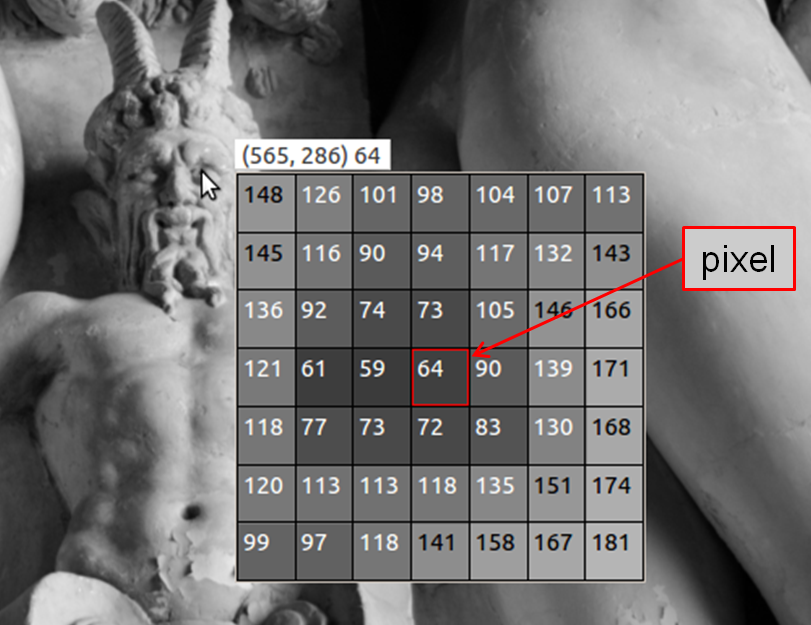
\includegraphics[width=4cm]{../graphics/faune.png}
        \caption{Grey level values around the left eye of the faun.}
      \end{figure}

    \end{column}
  \end{columns}

  \begin{alertblock}{}
   Designing computer vision systems that are able to extract semantic information from an image is a difficult task. How can we build systems that extract meaning from an image?
  \end{alertblock}

\end{frame}


%%%%%%%%%%%%%%%%%%%%%%%%%%%%%%%%%%%%
\begin{frame}{Extracting semantic information from an image}

\begin{columns}
  \begin{column}{.5\textwidth}
\begin{itemize}
\item Where is the phone? (localization task)
\item How many mugs are there? (quantification task)
\item Is there a window in the room?
\item At what time of the day was the photograph taken?
\end{itemize}
  \end{column}

  \begin{column}{.5\textwidth}
    \begin{figure}[ht]
      \centering
      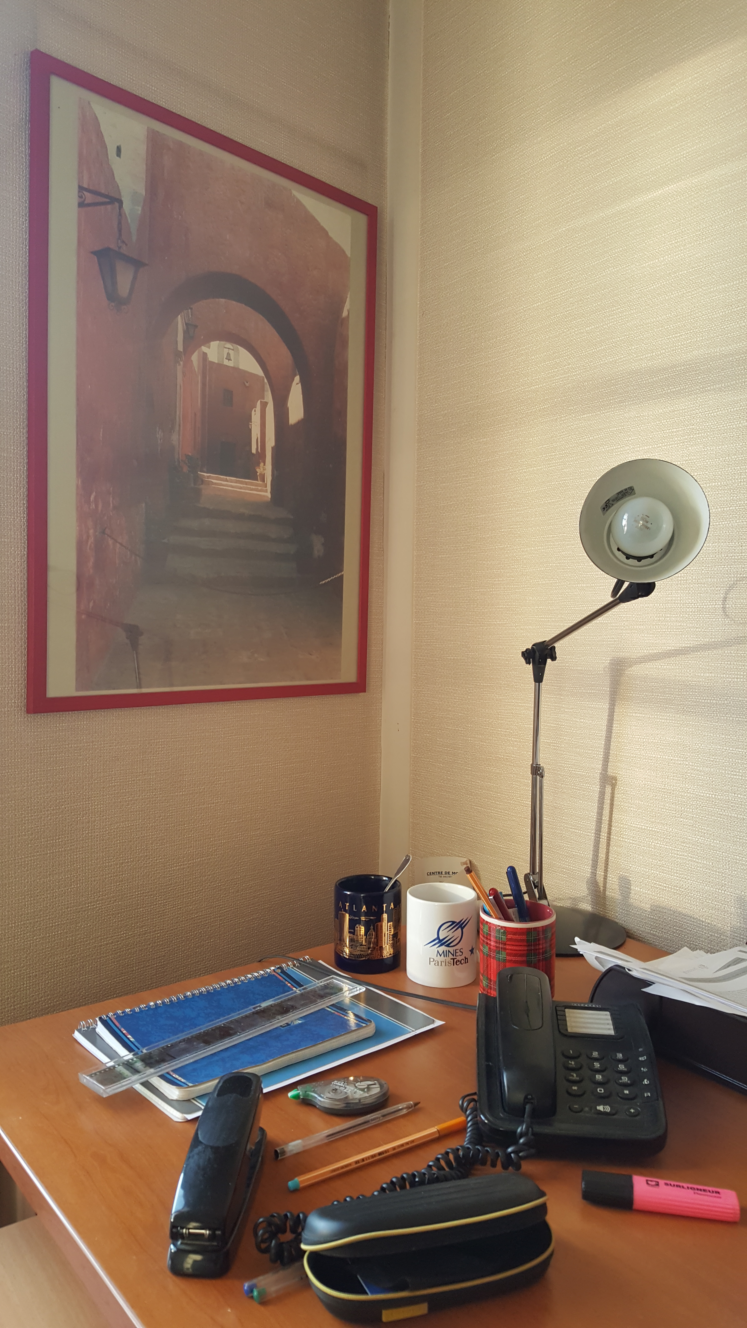
\includegraphics[height=8cm]{bureau-1}
    \end{figure}

  \end{column}
\end{columns}

\end{frame}


%%%%%%%%%%%%%%%%%%%%%%%%%%%%%%%%%%%%
\begin{frame}{Image processing approach}

  \begin{block}{}
    \begin{itemize}
    \item Build a mathematical model for the objects you are interested in
    \item Implement this model using image processing operators
    \end{itemize}
  \end{block}

\begin{itemize}
\item[+] This approach works correctly when the objects are not too complex.
\item[-] If objects are difficult to model, machine learning methods can bring a solution.
\end{itemize}


\end{frame}



%%%%%%%%%%%%%%%%%%%%%%%%%%%%%%%%%%%%
\frame{
\frametitle{Classical machine learning approach}

    \begin{block}{}
      \begin{itemize}
      \item Compute features from the image
      \item Apply machine learning to those features
      \end{itemize}
    \end{block}

\begin{itemize}
\item[+] Works well when you engineer the right features
\item[-] An expert is required to define those features - and this can be a long process
\item[-] Annotated data is required
\end{itemize}


}

%%%%%%%%%%%%%%%%%%%%%%%%%%%%%%%%%%%%
\begin{frame}{Deep learning approach}

  \begin{block}{Modern neural networks approach}
      \begin{itemize}
      \item Directly take as input the image pixels
      \item The network is supposed to build its own features
      \end{itemize}
    \end{block}

  \begin{itemize}
  \item[+] Good (impressive!) results
  \item[-] A large amount of annotated data is required
  \end{itemize}

\end{frame}

%%%%%%%%%%%%%%%%%%%%%%%%%%%%%%%%%%%%%%%%%%%%%%%%%%

\frame{
  \frametitle{Some accomplishments}

  \begin{block}{ImageNet Large Scale Visual Recognition Challenge (ILSVRC)}
    2012: \emph{AlexNet} \cite{krizhevsky_imagenet_2012} won this challenge by a large margin
    \end{block}

  The database contains more that 1 million training images, belonging to 1000 different classes (including 120 dog breeds!).


  }

%%%%%%%%%%%%%%%%%%%%%%%%%%%%%%%%%%%%%%%%%%%%%%%%%%

\frame{
  \frametitle{Some accomplishments (cont.)}

\begin{itemize}
\item 2011: first super-human performance, IJCNN 2011 traffic sign recognition contest \cite{ciresan_committee_2011}
\item 2012: visual object detection (Mitosis detection in breast cancer histology \cite{ciresan_mitosis_2013})
\item 2012: segmentation competition (neuronal membranes in electron microscopy images \cite{ciresan_deep_2012})
\item 2016: AlphaGo beats Lee Sedol, one of the best go players, in a 5-game match
\end{itemize}

}


%%%%%%%%%%%%%%%%%%%%%%%%%%%%%%%%%%%%
\begin{frame}{Deep learning applications with images}

\begin{itemize}
\item classification
\item object localization
\item semantic segmentation
\item instance segmentation
\item transformation (filtering, in-painting, editing, colorization…)
\item quantification
\item compression
\item image caption generation
\item 2D to 3D (stereo matching, 3D reconstruction, …)
\item motion estimation
\item Style transfer
\item Anomalous image detection
\item Image generation
\end{itemize}


\end{frame}



%%%%%%%%%%%%%%%%%%%%%%%%%%%%%%%%%%%%%%%%%%%%%%%%%%

\frame{
\frametitle{Convolutional neural networks in deep learning}

\begin{itemize}

%% \item They play a major role in deep learning
\item They are pivotal to many of the successes achieved by neural networks these recent years
\item They are interesting for dealing with regular structured data, such as images (or board games!)

\end{itemize}

\begin{block}{Acronyms}
  Two acronyms are used for convolutional neural networks in the literature: \emph{CNN} and \emph{ConvNet}.
  \end{block}

\begin{block}{Essential milestones}
  \begin{itemize}
  \item 1979: Neocognitron (CNN architecture) \cite{fukushima_neural_1979,fukushima_neocognitron:_1980}
  \item 1989: Backpropagation applied to CNNs \cite{lecun_backpropagation_1989}
  \item 2006, 2010: GPU implementation \cite{chellapilla_high_2006, ciresan_deep_2010}
  \end{itemize}
\end{block}

}

%%%%%%%%%%%%%%%%%%%%%%%%%%%%%%%%%%%%%%%%%%%%%%%%
\section{Application of fully-connected networks to image classification}

%%%%%%%%%%%%%%%%%%%%%%%%%%%%%%%%%%%%%%%%%%%%%%%%%%

\frame{
\frametitle{Artificial neuron}

\begin{figure}
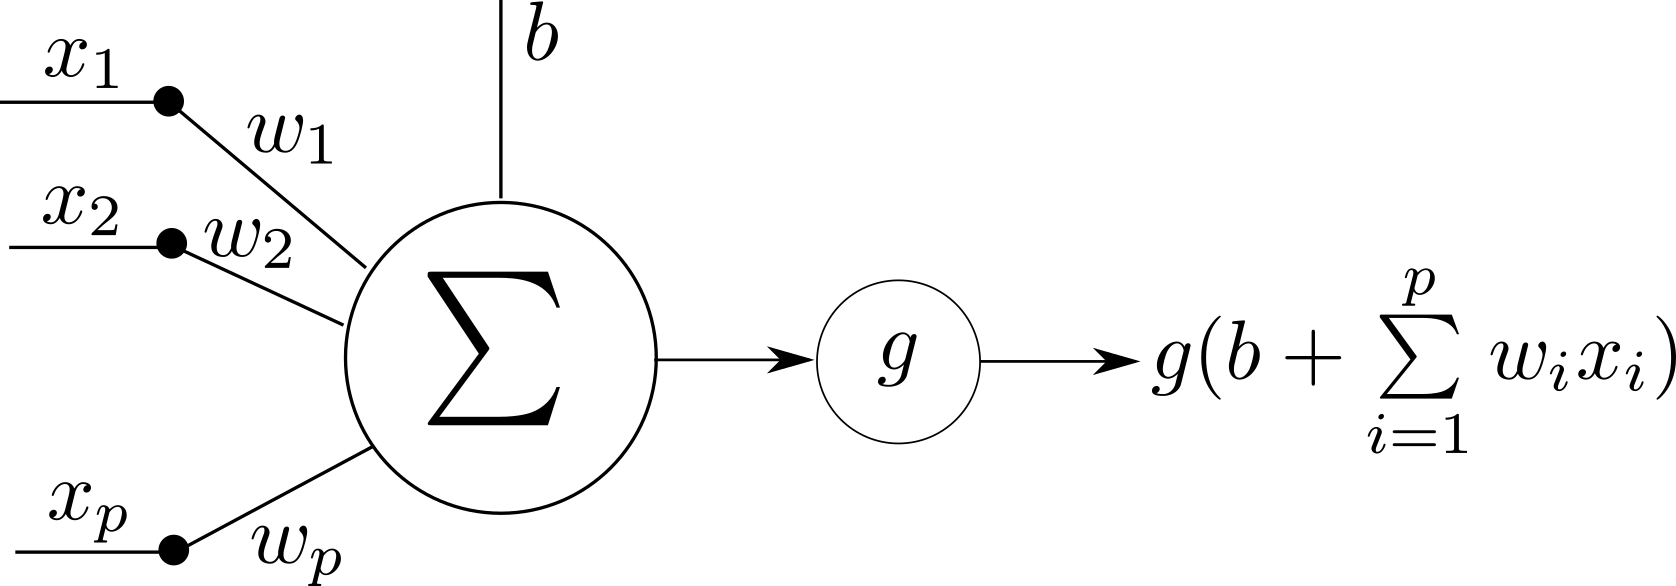
\includegraphics[height=3cm]{neurone}
\end{figure}

\begin{itemize}

\item $b, w_1, \ldots, w_n$ are the neuron parameters, to be learnt

\item $\act$ is the activation or transfer function

\end{itemize}


}

%%%%%%%%%%%%%%%%%%%%%%%%%%%%%%%%%%%%%%%%%%%%%%%%%%

\frame{
\frametitle{Neural network}


\begin{figure}
  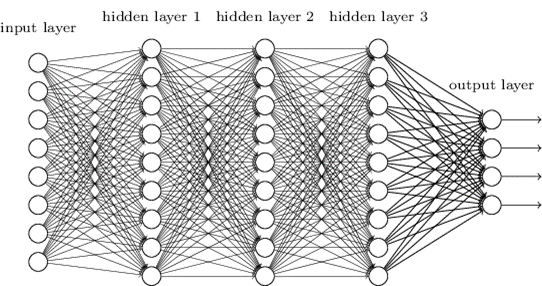
\includegraphics[height=5cm]{network}
\end{figure}

{\small(from http://www.jtoy.net)}

}


%%%%%%%%%%%%%%%%%%%%%%%%%%%%%%%%%%%%%%%%%%%%%%%%%%

\frame{
\frametitle{Input image, input neurons}

In the scalar case (single-valued images), each input pixel is considered as an input neuron.

\vspace{10pt}

\begin{columns}

  \begin{column}<1->{0.45\textwidth}
    \begin{center}
      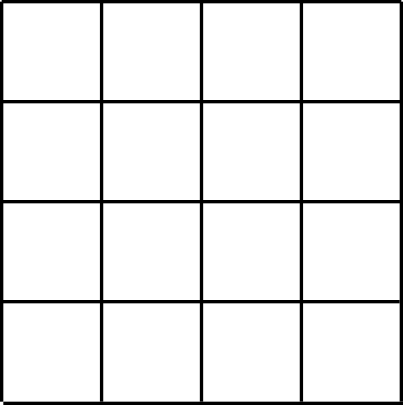
\includegraphics[width=0.50\textwidth]{image_as_pixels.png}
    \end{center}
  \end{column}

  \begin{column}<2->{0.45\textwidth}
    \begin{center}
      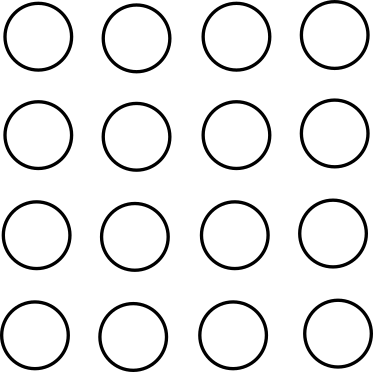
\includegraphics[width=0.50\textwidth]{image_as_neurons.png}

    \end{center}
  \end{column}

\end{columns}

}


%%%%%%%%%%%%%%%%%%%%%%%%%%%%%%%%%%%%
\begin{frame}{Image classification problem}

  Classification problem:
  \begin{itemize}
  \item Input: image $\x$
  \item Output: class $y \in \{ label_1, label_2, \ldots, label_q\}$
  \end{itemize}

\begin{block}{Class coding}
  Often, classes are denoted by integers, but this is only a coding commodity. For instance, it would be meaningless to use a regression approach for this problem.
\end{block}

\end{frame}

%%%%%%%%%%%%%%%%%%%%%%%%%%%%%%%%%%%%
\begin{frame}{Class coding}

  If there are $q$ possible classes, then a class will be coded as a vector $\y$ of length $q$. If its class is $r$  then for $0 \leq i < q$:
  \[
\y[i] =
    \begin{cases}
      1, & \text{if}\ i=r \\
      0, & \text{otherwise}
    \end{cases}
    \]

  \begin{block}{Example with $4$ classes}
    \begin{itemize}
    \item
    Label $0 \longmapsto [1,0,0,0]$
    \item
    Label $1 \longmapsto [0,1,0,0]$
    \item
    Label $2 \longmapsto [0,0,1,0]$
    \item
    Label $3 \longmapsto [0,0,0,1]$
    \end{itemize}
  \end{block}

\end{frame}


%%%%%%%%%%%%%%%%%%%%%%%%%%%%%%%%%%%%
\begin{frame}{Image classification with a neural network}

  \begin{block}{Input}
    Scalar image is transformed into a vector of length $p$.
  \end{block}

  \begin{block}{Output}
    For $q$ classes, the output will be a vector of length $q$.
  \end{block}

  \begin{block}{Example: image of size $4 \times 2$, $4$ possible classes}
    \begin{figure}
      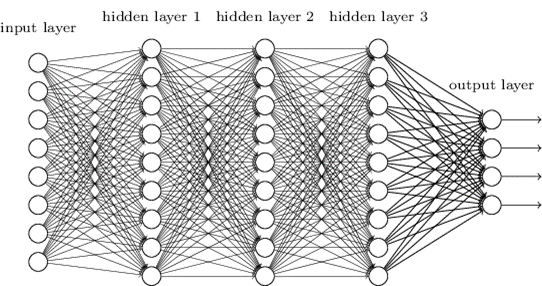
\includegraphics[width=0.5\textwidth]{network}
    \end{figure}
  \end{block}

\end{frame}


%%%%%%%%%%%%%%%%%%%%%%%%%%%%%%%%%%%%
\begin{frame}{Activation of the last layer}

\end{frame}

%%%%%%%%%%%%%%%%%%%%%%%%%%%%%%%%%%%%
\begin{frame}{Loss function for classification: cross-entropy}

\end{frame}

%%%%%%%%%%%%%%%%%%%%%%%%%%%%%%%%%%%%%%%%%%%%%%%%%%
\frame{
  \frametitle{Conclusion on fully-connected networks for image classification}

Fully connected layers:

\begin{itemize}

\item scale badly to large size images

\item do not take into account the local structure of images

\end{itemize}


Today:

\begin{itemize}
\item Fully-connected networks are almost never used for image analysis.
\item Fully-connected layers are only used in the middle (auto-encoders) or at the end (classification) of the pipeline.
\end{itemize}

}



%%%%%%%%%%%%%%%%%%%%%%%%%%%%%%%%%%%%%%%%%%%%%%%%%%
%%%%%%%%%%%%%%%%%%%%%%%%%%%%%%%%%%%%%%%%%%%%%%%%%%
\section{From fully-connected layers to convolutional layers}



%%%%%%%%%%%%%%%%%%%%%%%%%%%%%%%%%%%%%%%%%%%%%%%%%%
\frame{
\frametitle{Towards convolutional layers}


\begin{block}{}
In the following slides, for illustration purposes, we will consider one-dimensional images
\end{block}


\begin{columns}

  \begin{column}<1->{0.3\textwidth}
    \begin{center}
      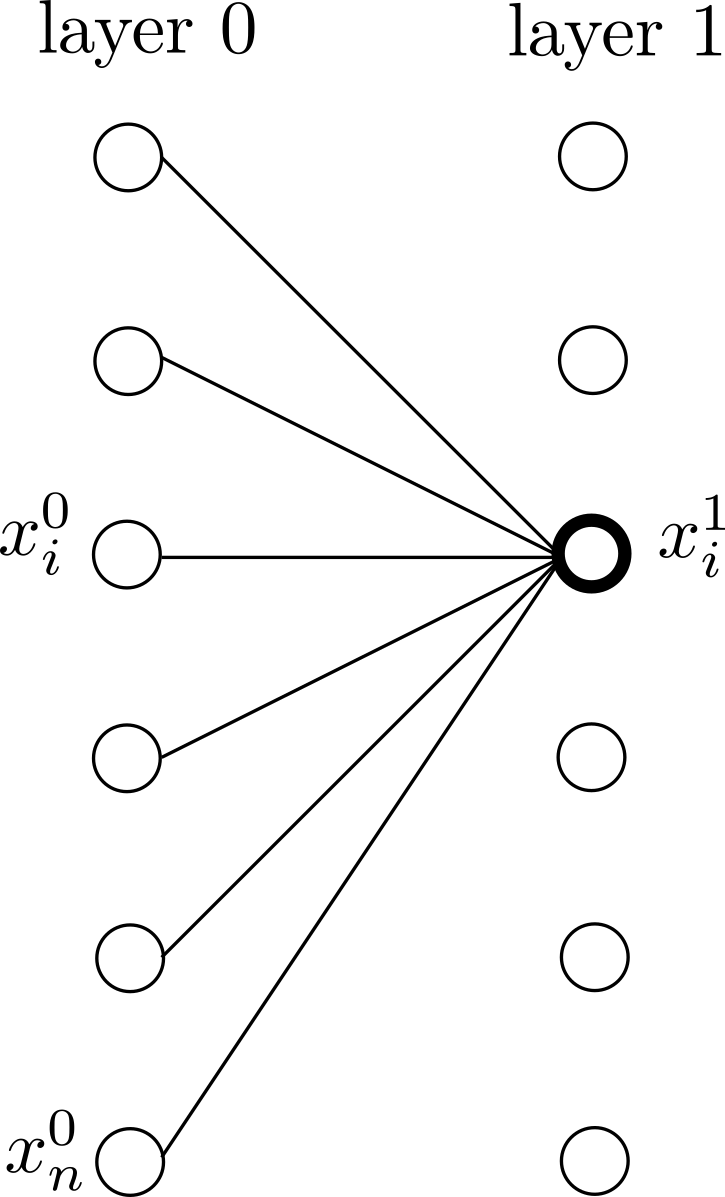
\includegraphics[width=0.74\textwidth]{fully_connected_layer.png}
      \\Fully connected layer: $n(s+1)$ weights
    \end{center}
  \end{column}

  \begin{column}<2->{0.3\textwidth}
    \begin{center}
      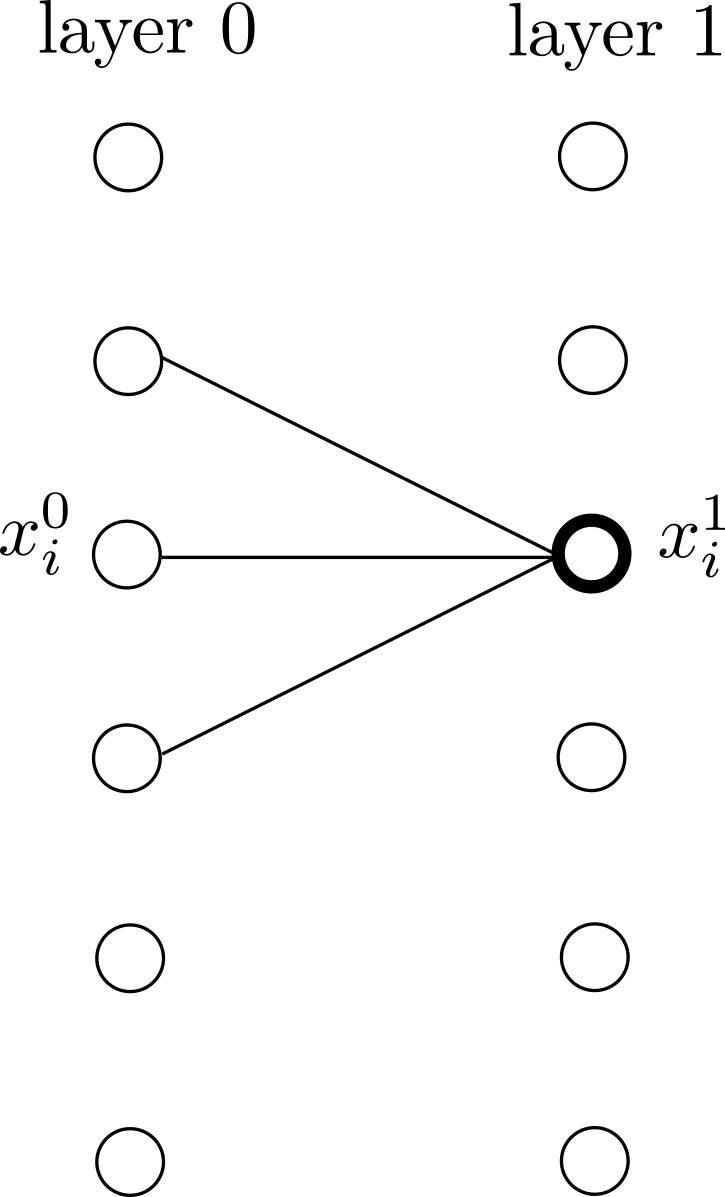
\includegraphics[width=0.74\textwidth]{locally_connected_layer.png}
      \\Locally conn. layer: $n(s+1)$ weights
    \end{center}
  \end{column}

  \begin{column}<3->{0.3\textwidth}
    \begin{center}
      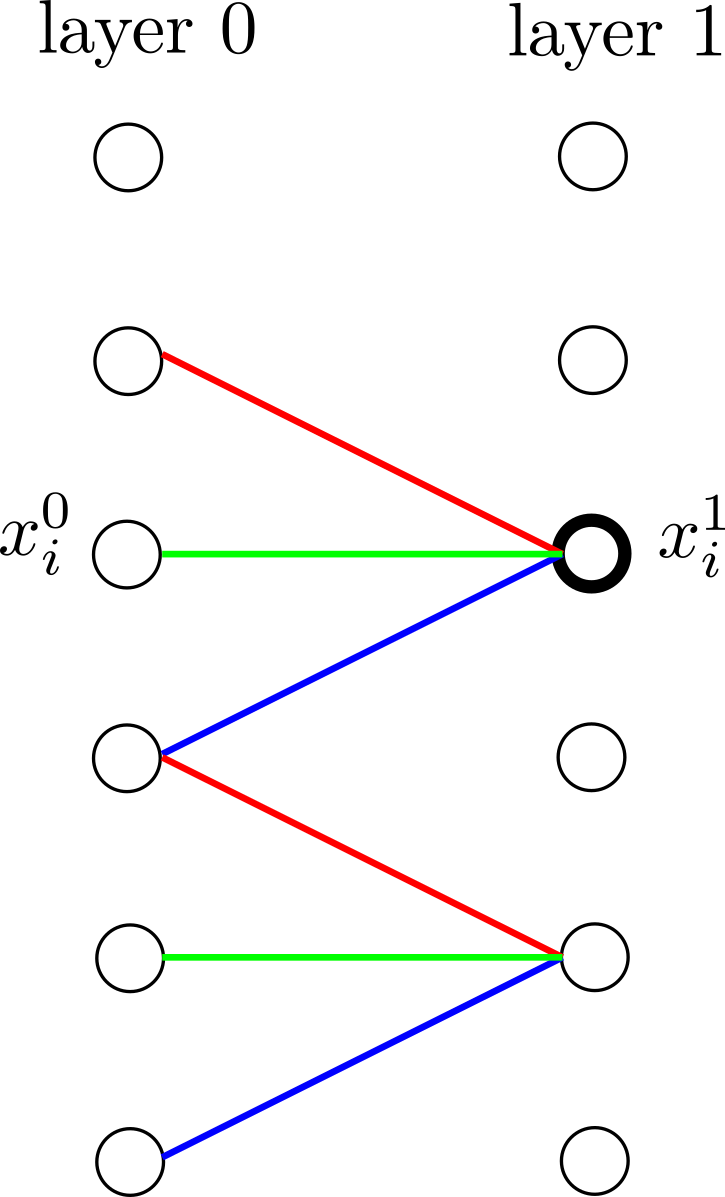
\includegraphics[width=0.74\textwidth]{convolutional_layer.png}
      \\Weight replication: $s+1$ weights
    \end{center}
  \end{column}

\end{columns}

\begin{block}<4->{}
  A convolutional layer computes a convolution, plus a constant, of the precedent layer.
\end{block}


}


%%%%%%%%%%%%%%%%%%%%%%%%%%%%%%%%%%%%%%%%%%%%%%%%%%
\frame{
\frametitle{Stride}

A convolutional layer can at the same time downsample the image by applying a sampling step, or \emph{stride}.

\begin{columns}

  \begin{column}<1->{0.3\textwidth}
    \begin{center}
      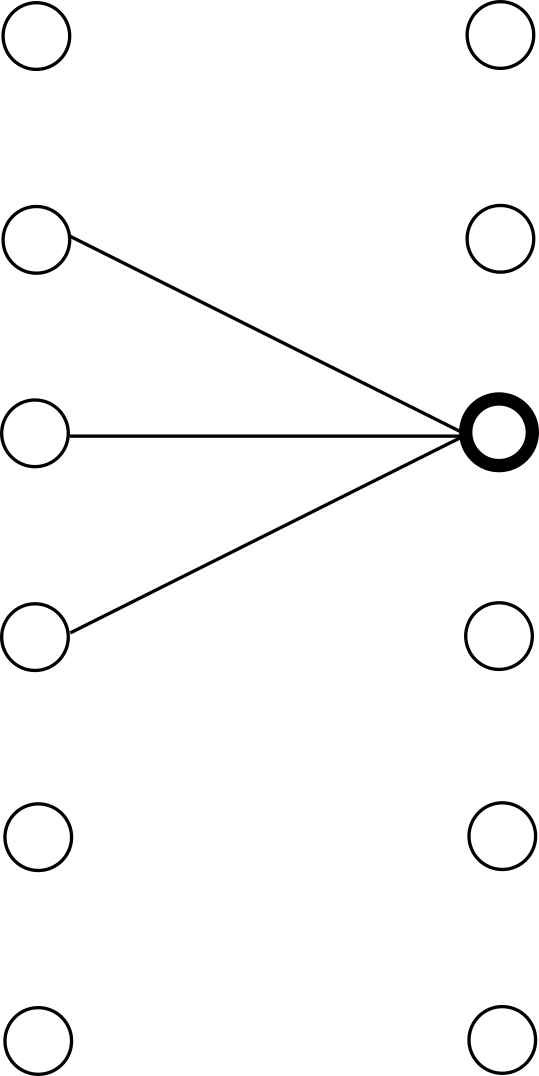
\includegraphics[width=0.60\textwidth]{stride1.png}
      \\Stride 1
    \end{center}
  \end{column}

  \begin{column}<2->{0.3\textwidth}
    \begin{center}
      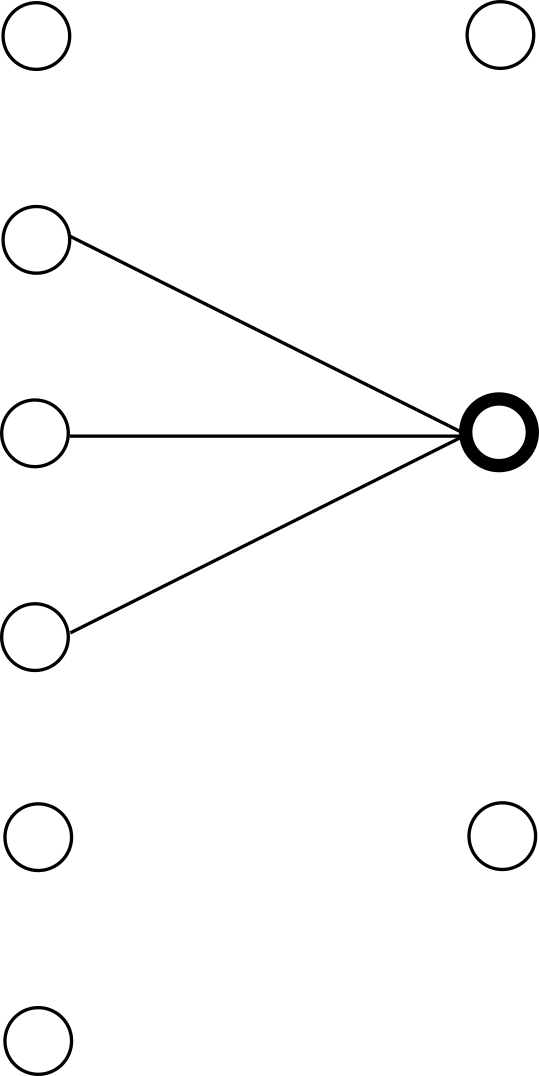
\includegraphics[width=0.60\textwidth]{stride2.png}
      \\Stride 2
    \end{center}
  \end{column}

  \begin{column}<3>{0.3\textwidth}
    \begin{center}
      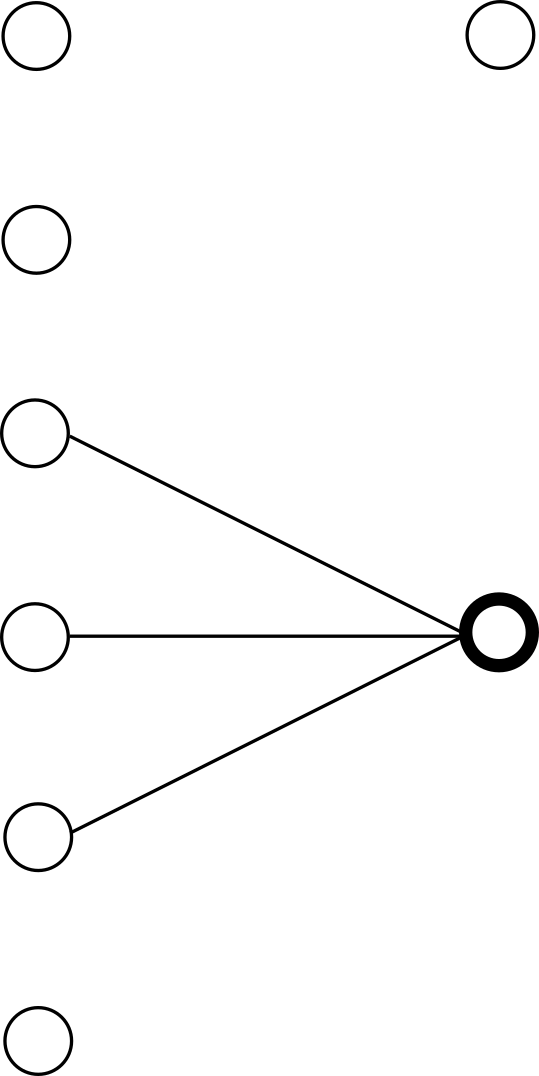
\includegraphics[width=0.60\textwidth]{stride3.png}
      \\Stride 3
    \end{center}
  \end{column}

\end{columns}


}

%%%%%%%%%%%%%%%%%%%%%%%%%%%%%%%%%%%%%%%%%%%%%%%%%%
\frame{
\frametitle{Several filters in the same convolutional layer}

    \begin{center}
      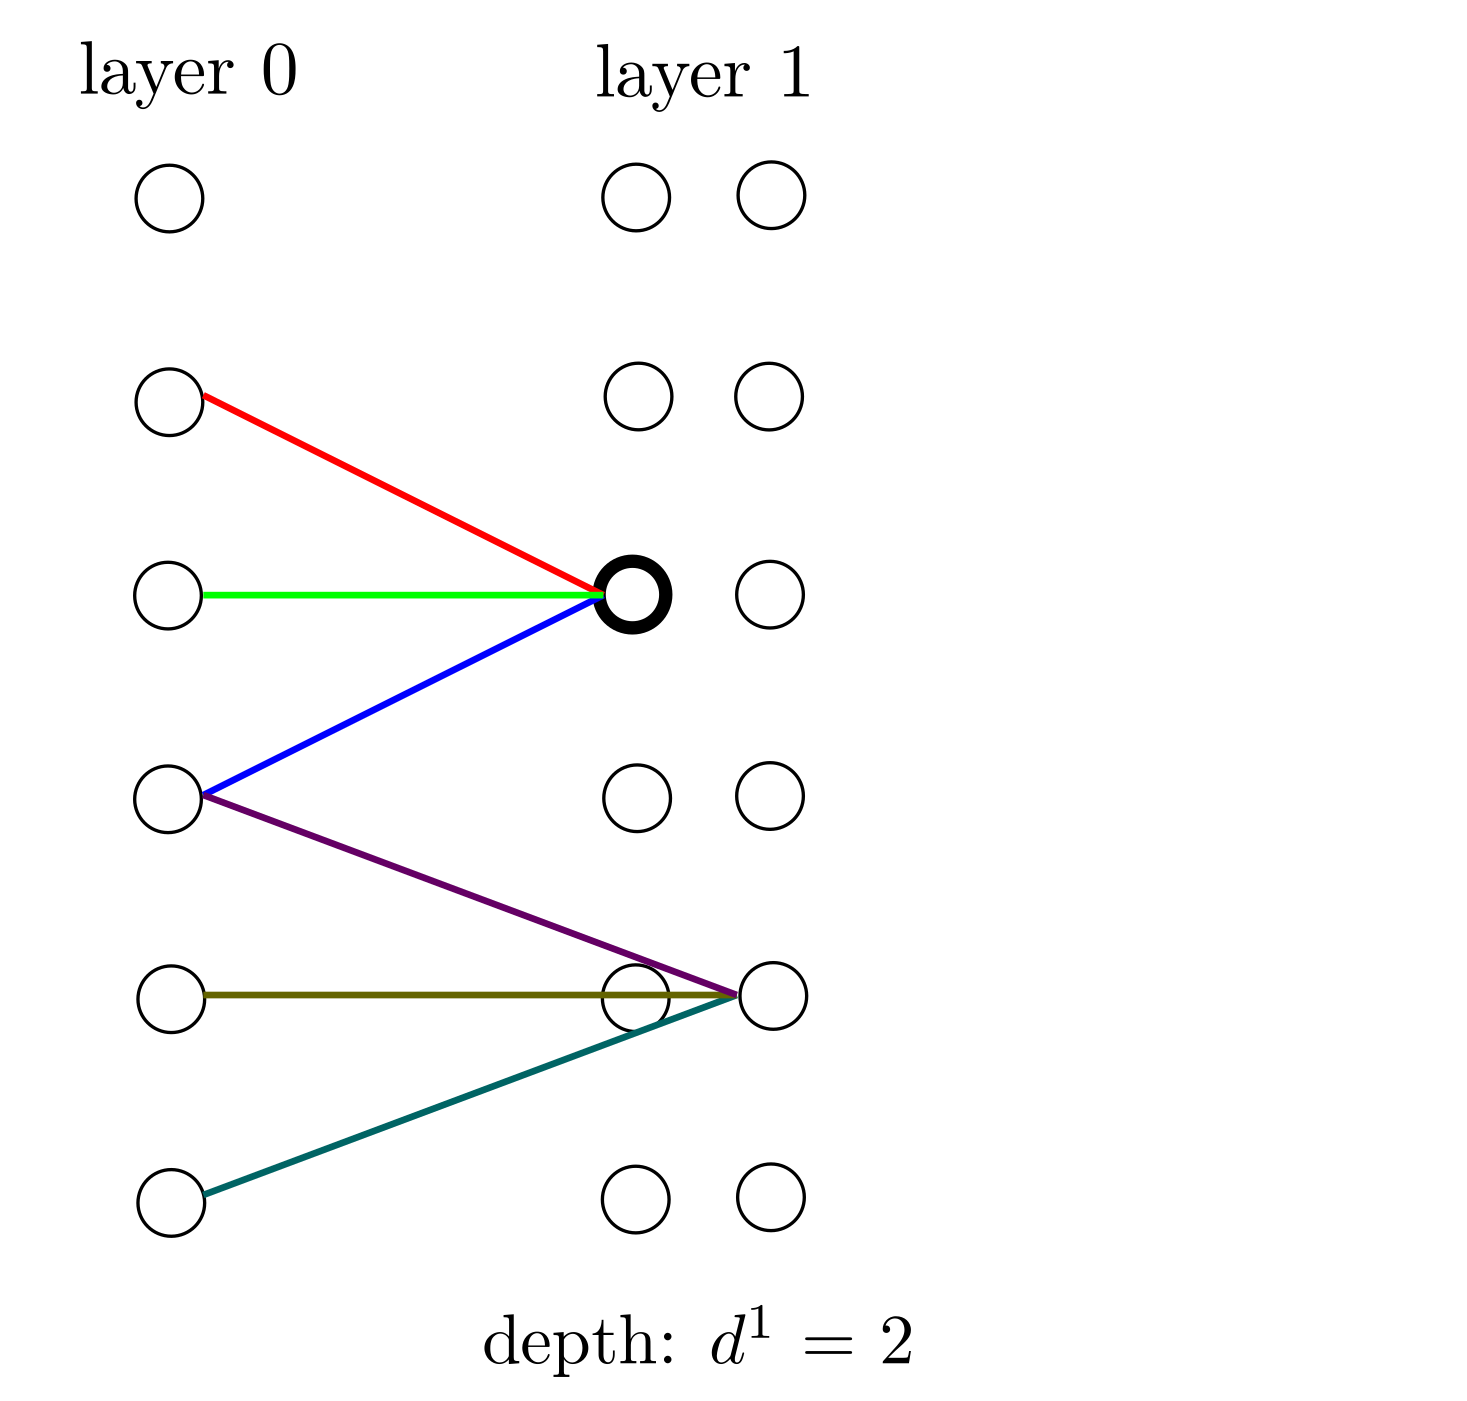
\includegraphics[width=0.53\textwidth]{convolutional_layer2.png}

    \end{center}


}

%%%%%%%%%%%%%%%%%%%%%%%%%%%%%%%%%%%%%%%%%%%%%%%%%%
\frame{
\frametitle{Several filters in the same convolutional layer}

    \begin{center}
      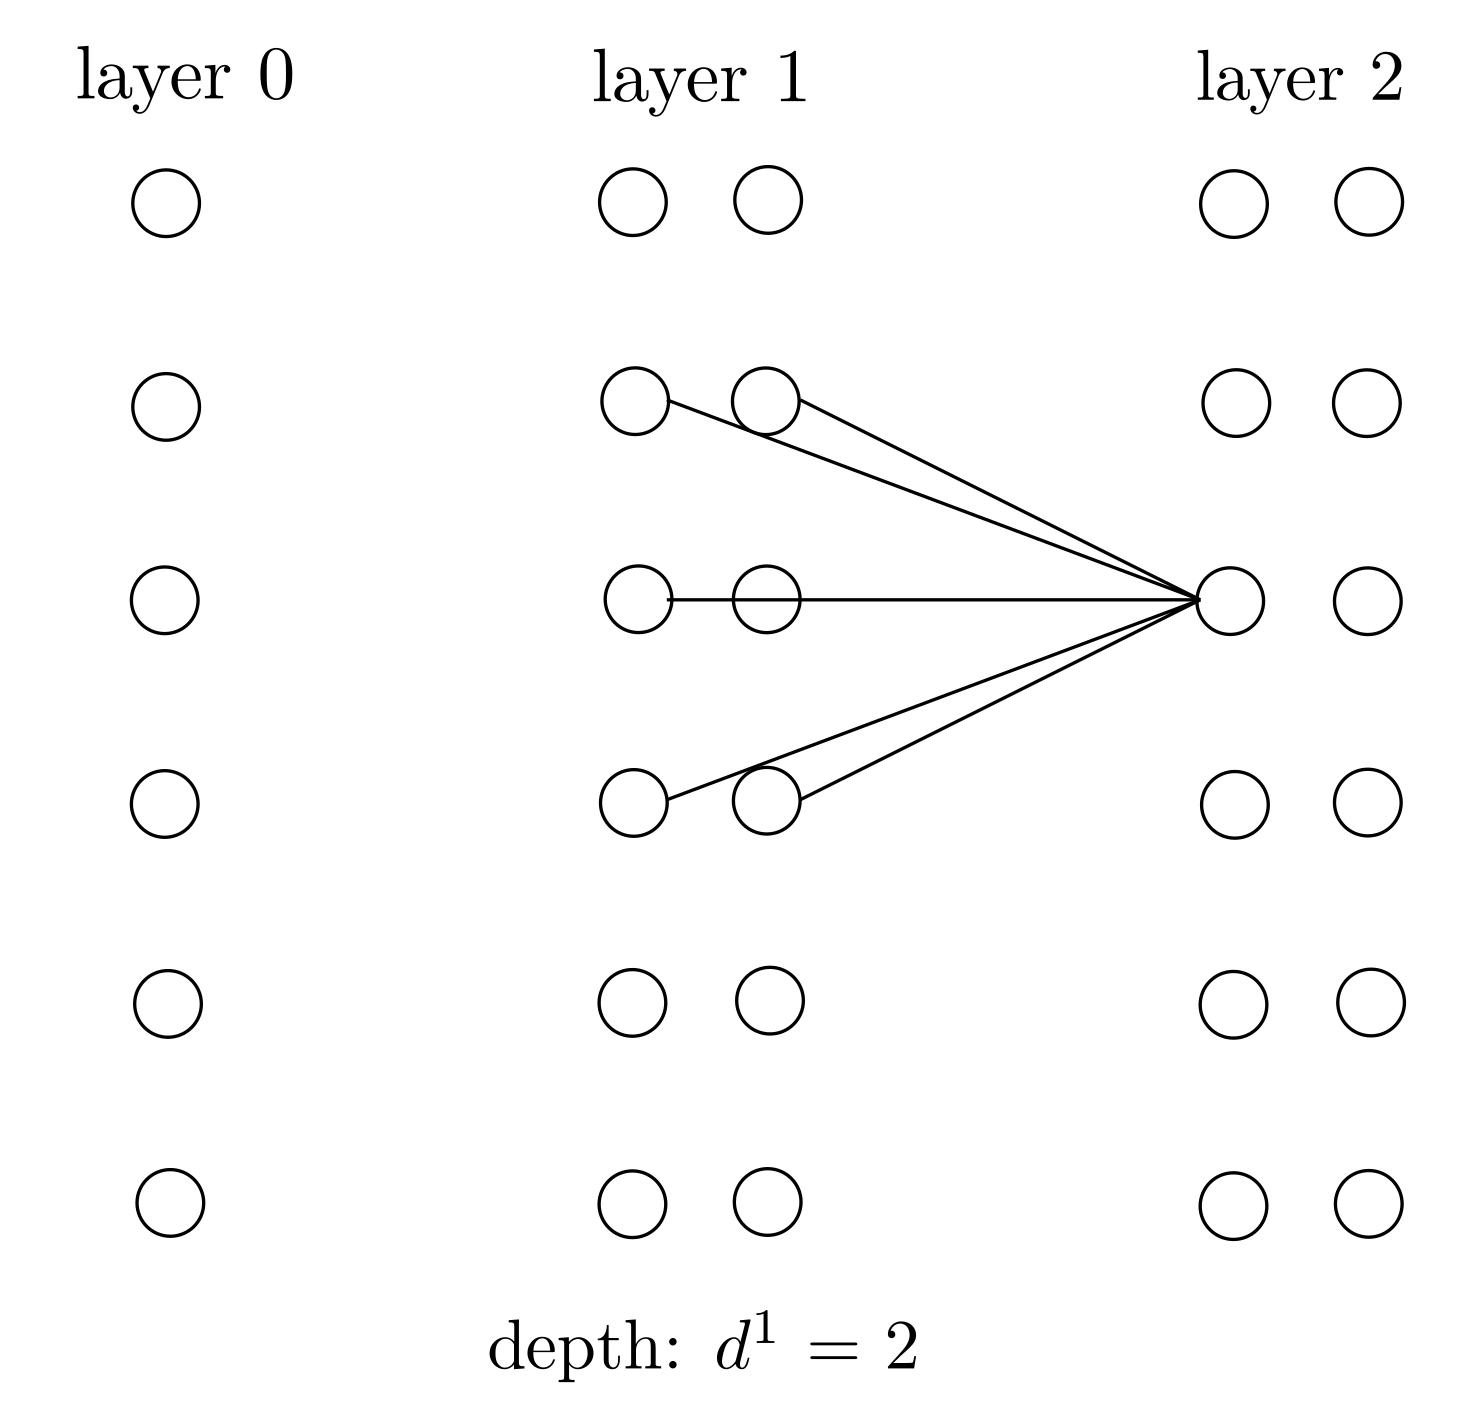
\includegraphics[width=0.53\textwidth]{convolutional_layer3.png}

    \end{center}


}

%%%%%%%%%%%%%%%%%%%%%%%%%%%%%%%%%%%%%%%%%%%%%%%%%%
\frame{
\frametitle{Several filters in the same convolutional layer}

    \begin{center}
      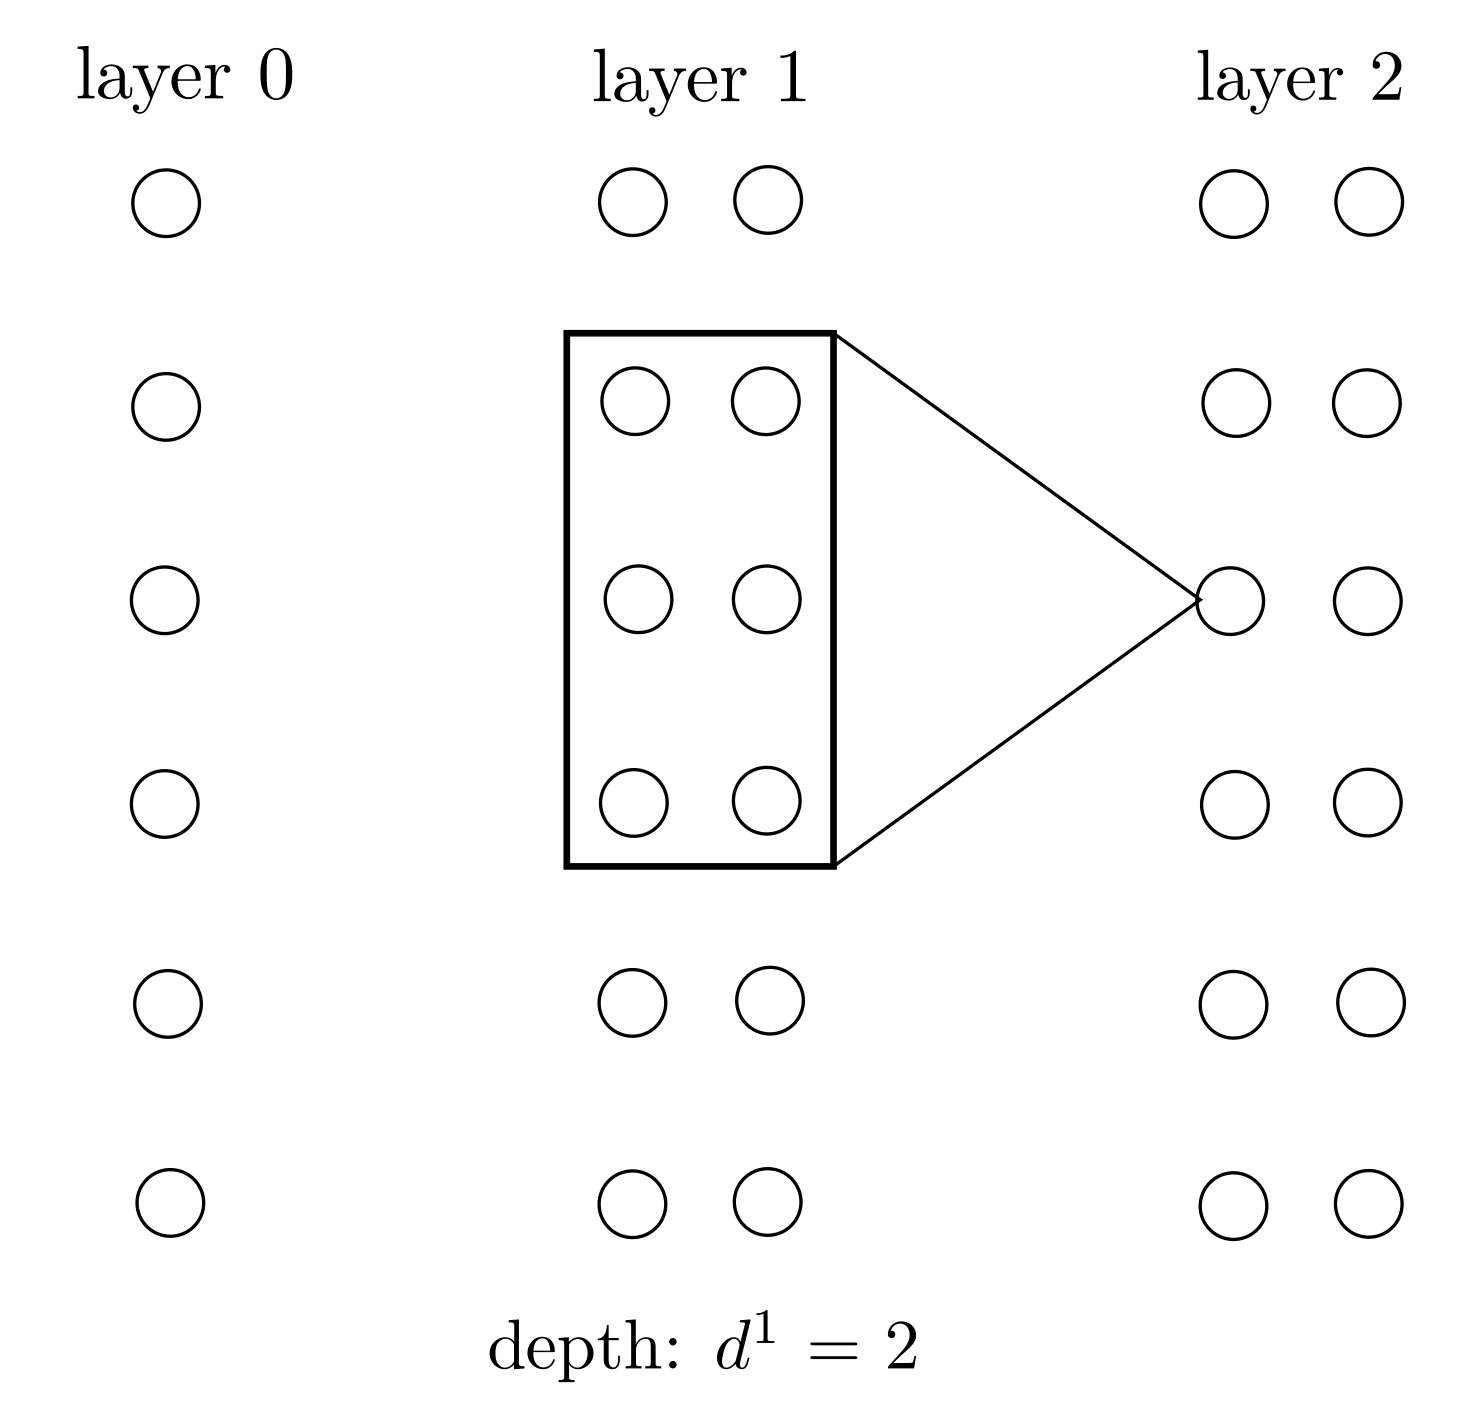
\includegraphics[width=0.53\textwidth]{convolutional_layer4.png}

    \end{center}


}

%%%%%%%%%%%%%%%%%%%%%%%%%%%%%%%%%%%%%%%%%%%%%%%%%%
\frame{
\frametitle{Consequences on the parameter number}

\begin{center}
  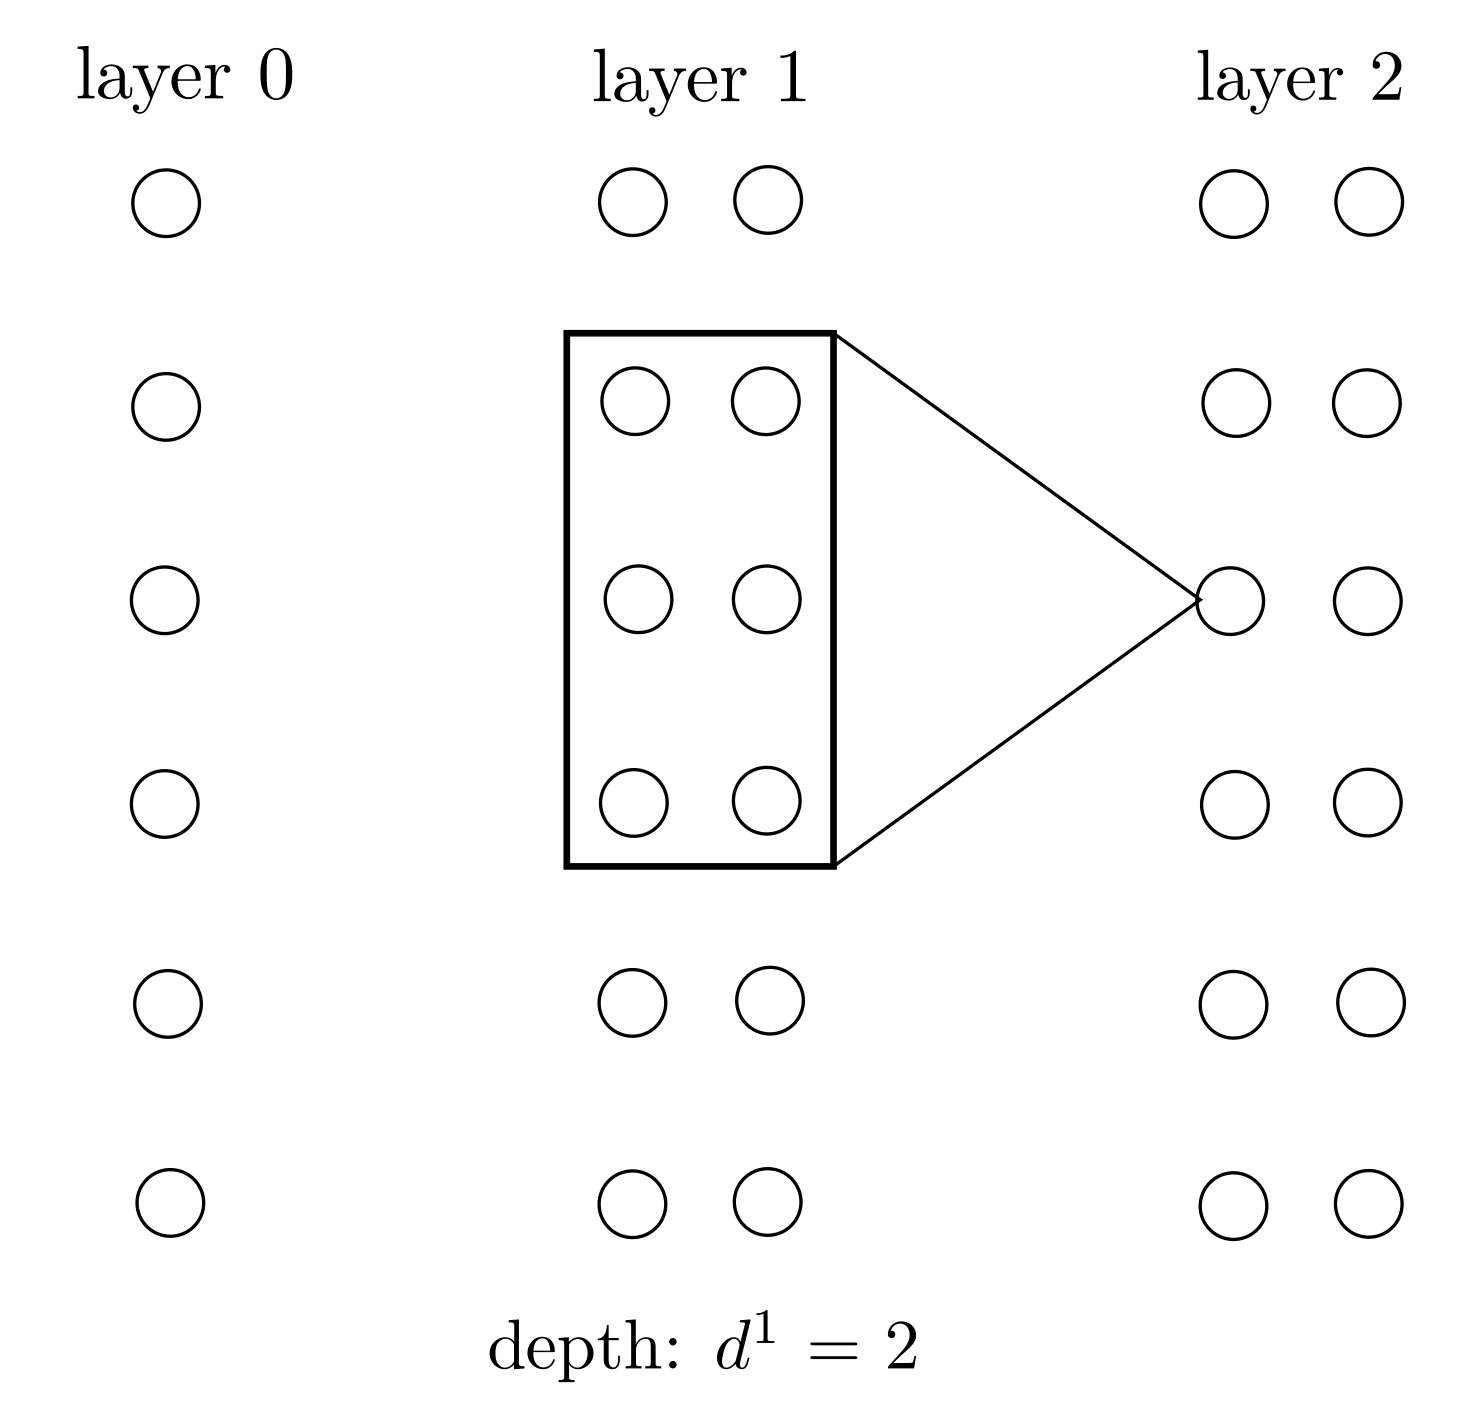
\includegraphics[width=0.5\textwidth]{convolutional_layer4.png}
\end{center}

\begin{itemize}
\item<1-> How many parameters do we have in layer 1?
\item<2-> $d^1 \times (s + 1)$
\item<3-> In layer 2?
\item<4-> $d^2 \times (d^1 \times s + 1)$
\end{itemize}

}




%%%%%%%%%%%%%%%%%%%%%%%%%%%%%%%%%%%%%%%%%%%%%%%%%%
\frame{
\frametitle{Multi-valued images}


An input image with $p$ channels (for instance à colour image with 3 channels) can be represented by an input layer of depth 3

\begin{center}
  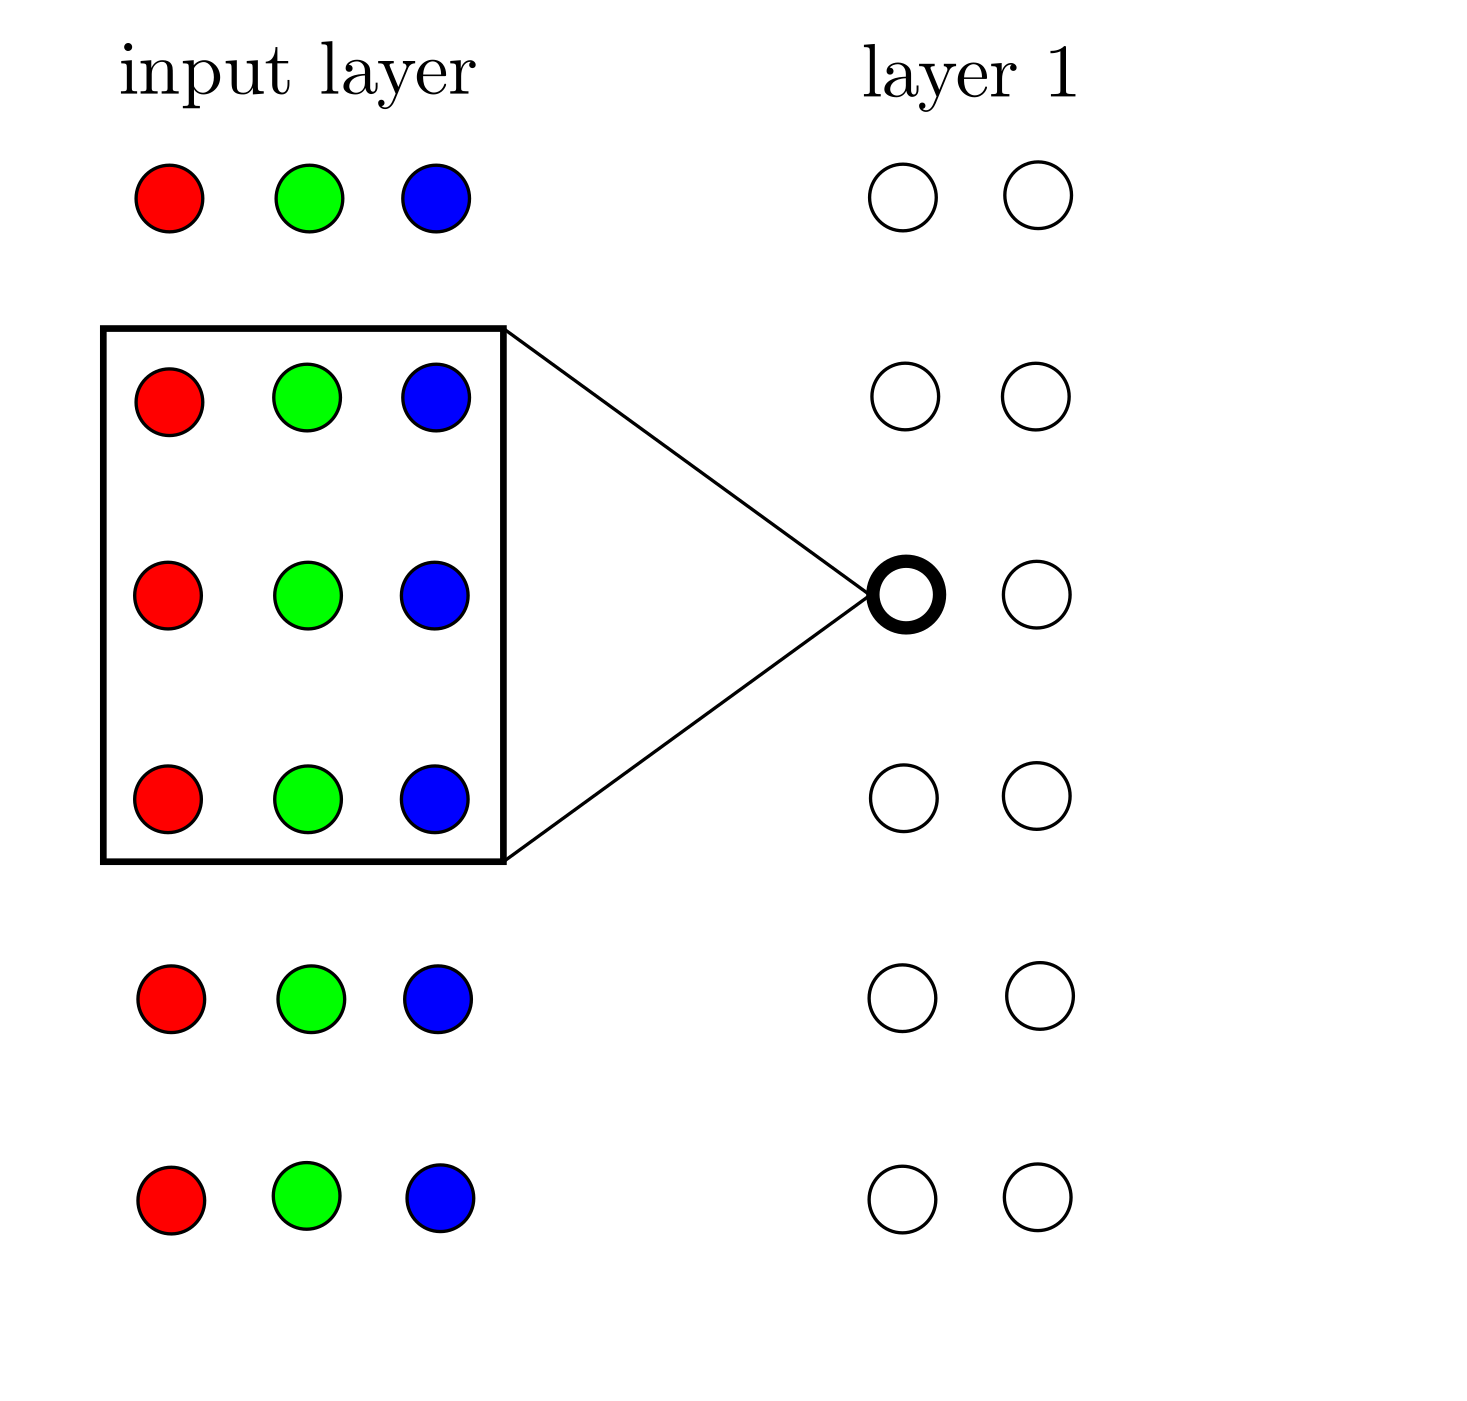
\includegraphics[width=0.31\textwidth]{input_vector_image.png}
\end{center}



}


%%%%%%%%%%%%%%%%%%%%%%%%%%%%%%%%%%%%%%%%%%%%%%%%%%
\frame{
\frametitle{Some properties}

\begin{itemize}
  \item Translation invariance
  \item Efficient implementation using matrix operations and graphical processing units
\end{itemize}

}


%%%%%%%%%%%%%%%%%%%%%%%%%%%%%%%%%%%%%%%%%%%%%%%%%%
%%%%%%%%%%%%%%%%%%%%%%%%%%%%%%%%%%%%%%%%%%%%%%%%%%
\section{Building convolutional networks}

%%%%%%%%%%%%%%%%%%%%%%%%%%%%%%%%%%%%%%%%%%%%%%%%%%

\frame{
\frametitle{Max pooling}

\begin{itemize}
\item Convolutional networks often contain subsampling steps. These can be done using strides of 2 or more within convolutional layers or, as it is common practice today, using \emph{max pooling} layers.

\item Sampling is only applied along the spatial dimensions, not along the dimension of the filters.

  \end{itemize}

\begin{center}
  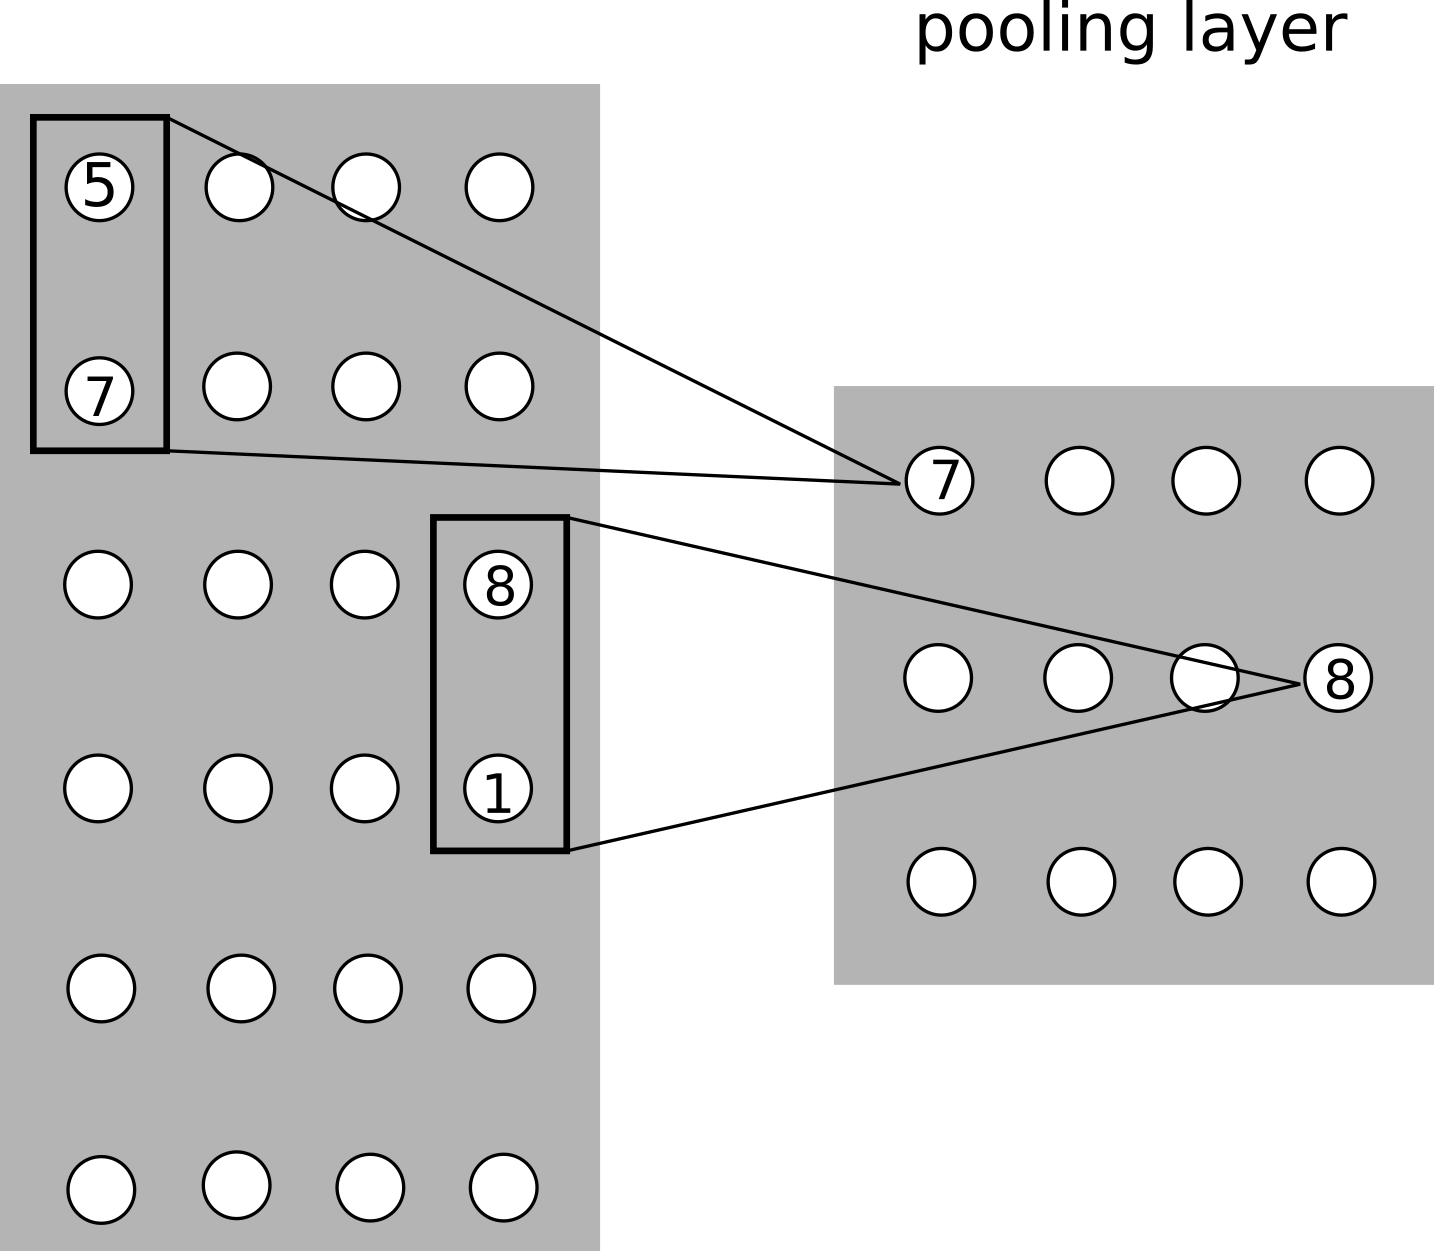
\includegraphics[width=0.41\textwidth]{max_pooling.png}
\end{center}


}


%%%%%%%%%%%%%%%%%%%%%%%%%%%%%%%%%%%%
\begin{frame}{Skip connections}

\end{frame}
%%%%%%%%%%%%%%%%%%%%%%%%%%%%%%%%%%%%%%%%%%%%%%%%%%

\frame{
\frametitle{Main components of a convolutional neural network}

Many successful architectures, especially for image classification, follow the same pattern:

\begin{enumerate}
\item Several iterations of: One or several convolutional layers, with increasing depth, followed by max pooling
\item A few fully connected layers
\end{enumerate}

}

%% %%%%%%%%%%%%%%%%%%%%%%%%%%%%%%%%%%%%%%%%%%%%%%%%%%

%% \frame{
%% \frametitle{Example networks: fovea detection}

%%   \begin{center}
%%   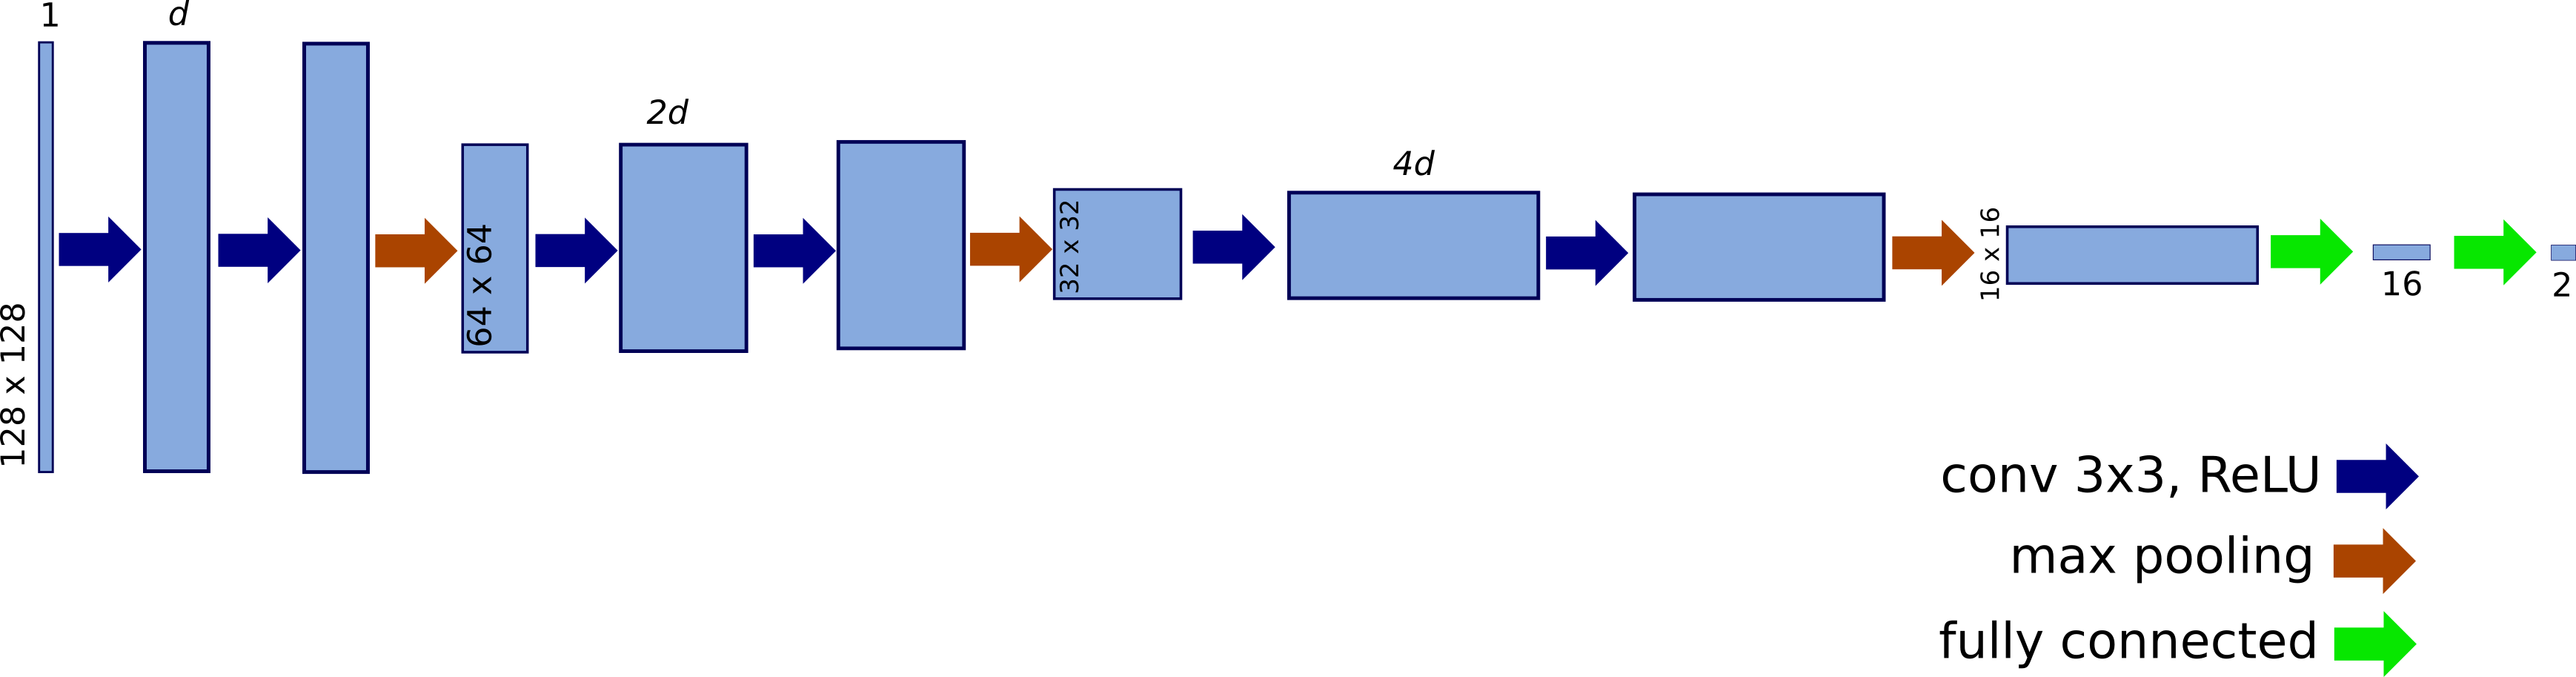
\includegraphics[width=\textwidth]{fovea_convnet2.png}
%% \end{center}

%%   }

%%%%%%%%%%%%%%%%%%%%%%%%%%%%%%%%%%%%%%%%%%%%%%%%%%

%% \frame{
%% \frametitle{A typical convolutional architecture for image classification}

%% \begin{figure}
%%   \includegraphics[width=9.5cm]{conv_net_classif}
%%   \caption{Architecture used for the classification of the NORB dataset (from \cite{scherer_evaluation_2010})}
%% \end{figure}

%% Note that layer P4 can be seen as made of features, which are then classified by the two fully connected layers.


%% }

%%%%%%%%%%%%%%%%%%%%%%%%%%%%%%%%%%%%%%%%%%%%%%%%%

\frame{
  \frametitle{VGGnet}


  \begin{itemize}
  \item Proposed by K. Simonyan and A. Zisserman from the University of Oxford \cite{simonyan_very_2014}
  \item Runner-up in the ImageNet Large Scale Visual Recognition Competition (ILSVRC) in 2014.

  \item Number of parameters (VGG16): $138$ million.

   \end{itemize}

  \begin{center}
    \begin{figure}
    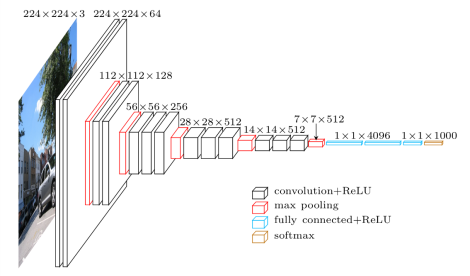
\includegraphics[width=0.65\textwidth]{vgg16.png}
    \caption{\tiny{VGG16 (From https://www.cs.toronto.edu/~frossard/post/vgg16/)}}
    \end{figure}
\end{center}


}



%%%%%%%%%%%%%%%%%%%%%%%%%%%%%%%%%%%%%%%%%%%%%%%%%

\frame{
  \frametitle{GoogLeNet (a.k.a. Inception v1)}


  \begin{itemize}

  \item Winner of the ImageNet Large Scale Visual Recognition Competition (ILSVRC) in 2014.

  \item Number of parameters: \emph{only} $~5$ million.

  \end{itemize}

\begin{figure}[ht]
  \centering
    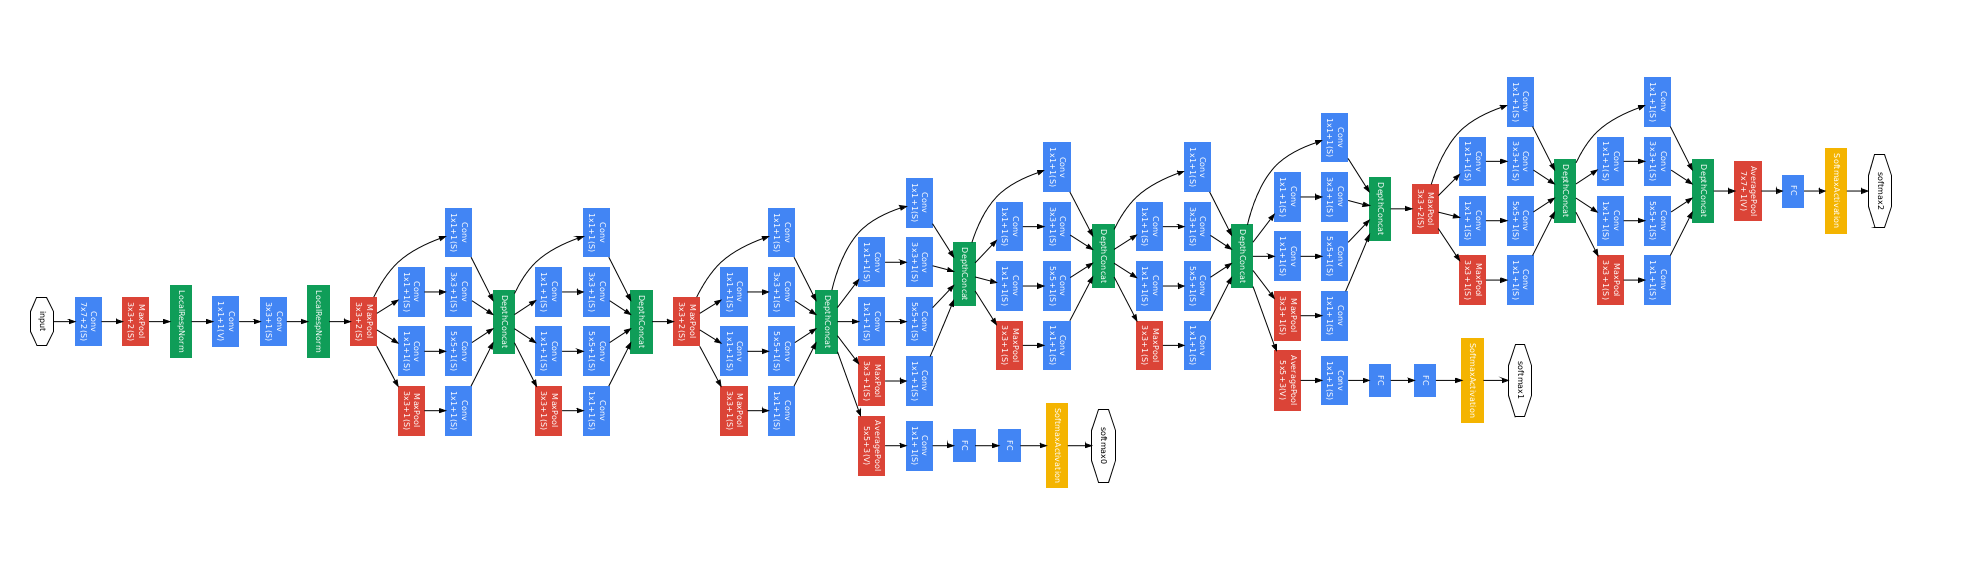
\includegraphics[width=\textwidth]{googlenet.png}
    \caption{\tiny{From \cite{szegedy_going_2014}}}
\end{figure}

  ResNet won the following year...

}


%%%%%%%%%%%%%%%%%%%%%%%%%%%%%%%%%%%%
\begin{frame}{Inception module}

\begin{figure}[ht]
  \centering
  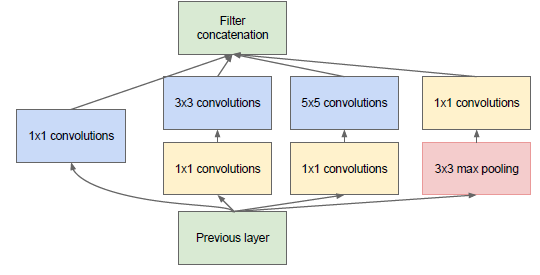
\includegraphics[width=0.75\textwidth]{inception_module.png}
  \caption{\tiny{From \cite{szegedy_going_2014}}}
\end{figure}

\end{frame}

%%%%%%%%%%%%%%%%%%%%%%%%%%%%%%%%%%%%
\begin{frame}{ResNet}

\begin{columns}
  \begin{column}{.5\textwidth}
\begin{itemize}
  \item Winner of the ImageNet Large Scale Visual Recognition Competition (ILSVRC) in 2015.
  \item The authors tested up to 1202 layers. They reported no training difficulties, but overfitting \cite{he_deep_2015}
\end{itemize}

  \end{column}

  \begin{column}{.5\textwidth}
\begin{figure}[ht]
  \centering
  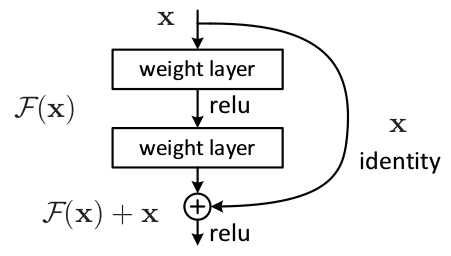
\includegraphics[width=\textwidth]{resnet_module.png}
  \caption{Residual learning block \tiny{(from \cite{he_deep_2015})}}
\end{figure}

  \end{column}
\end{columns}


\begin{figure}[ht]
  \centering
  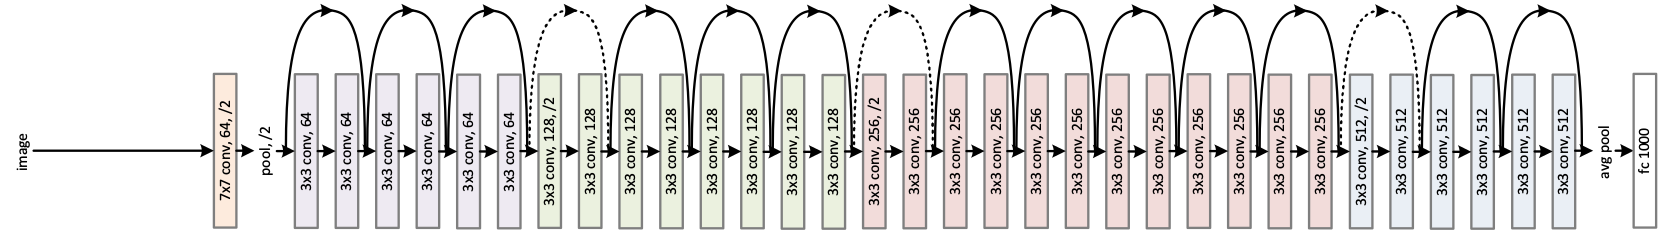
\includegraphics[width=\textwidth]{resnet.png}
  \caption{Residual network with 34 layers \tiny{(from \cite{he_deep_2015})} }
\end{figure}


\end{frame}


%%%%%%%%%%%%%%%%%%%%%%%%%%%%%%%%%%%%%%%%%%%%%%%%%%

\frame{
\frametitle{Current trends}

\begin{itemize}
\item Small convolutions ($3\times3$)
\item Dimension reduction using $1 \times 1$ convolutions
\item Increasing number of layers
\item Skip connections
\end{itemize}

}

%%%%%%%%%%%%%%%%%%%%%%%%%%%%%%%%%%%%%%%
\section{Practical considerations}

%%%%%%%%%%%%%%%%%%%%%%%%%%%%%%%%%%%%%%%%%%%%%%%%%%

\frame{
\frametitle{Designing a convolutional neural network}

\begin{itemize}
\item Network architecture
\item Hyper-parameter setting
\item Optimization method and parameters
\end{itemize}


\begin{block}{}
  Learning, specially for complex networks, can be difficult. It is always time consuming.
  \end{block}

}




%%%%%%%%%%%%%%%%%%%%%%%%%%%%%%%%%%%%%%%%%%%%%%%%%%

\frame{
\frametitle{Using an existing network}

\begin{itemize}
\item Replicate network architecture and hyper-parameters
\item Load weights
\end{itemize}

\begin{block}{}
  With standard libraries this is very simple. Prediction time is usually fast.
  \end{block}


}




%%%%%%%%%%%%%%%%%%%%%%%%%%%%%%%%%%%%%%%%%%%%%%%%%%

\frame{
\frametitle{ConvNets can be fooled}


Deep learning can produce astonishing results \cite{nguyen_deep_2015}...
\begin{figure}
  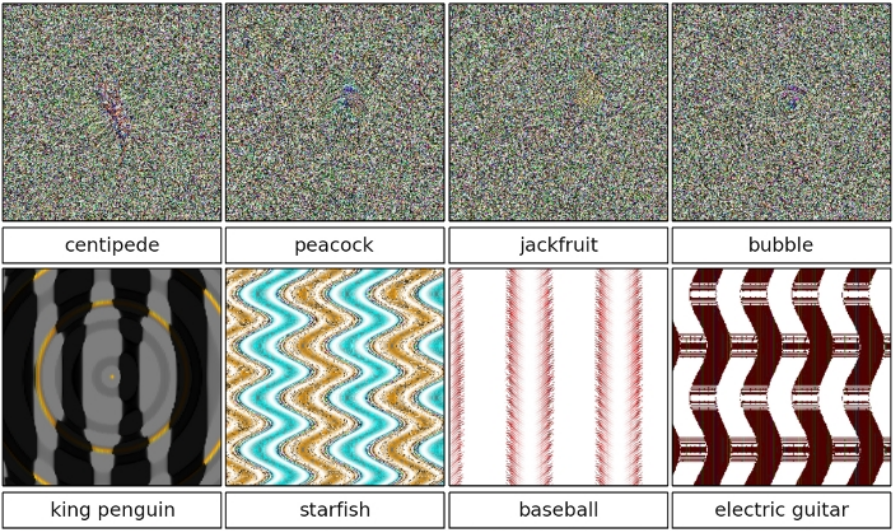
\includegraphics[width=0.8\textwidth]{dl_easily_fooled.png}
\end{figure}


}


%%%%%%%%%%%%%%%%%%%%%%%%%%%%%%%%%%%%%%%%%%%%%%%%%%

\frame{
\frametitle{Main deep learning libraries}

Deep learning is a very competitive domain, where code sharing is very common.

\begin{itemize}
\item Theano
\item Torch
\item Tensorflow
\item Caffe
\item MatConvNet
\end{itemize}

\begin{block}{Keras}
  Keras is a very easy to use interface to Theano and Tensorflow.
  \end{block}


}

%%%%%%%%%%%%%%%%%%%%%%%%%%%%%%%%%%%%%%%
\section{Visualization}

%%%%%%%%%%%%%%%%%%%%%%%%%%%%%%%%%%%%%%%%%%%%%%%%%%

\frame{
  \frametitle{Visualizing at least what we don't understand}

  We do not fully understand today where the good performances of deep learning come from. But we can at least have a look at what is going on inside the networks.

  \begin{itemize}
  \item Neuron outputs (activations)
  \item Filter values
  \item ``Important'' pixels
    \end{itemize}


}

%%%%%%%%%%%%%%%%%%%%%%%%%%%%%%%%%%%%%%%%%%%%%%%%%%

\frame{
  \frametitle{Maximal neuron activation}

Which images maximally activate a given neuron? \cite{girshick_rich_2014}

\begin{figure}
  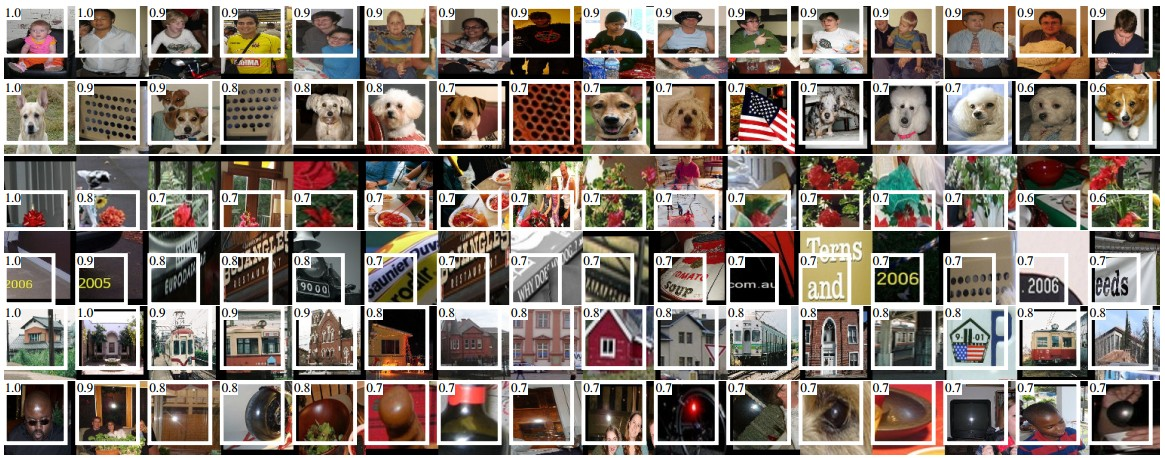
\includegraphics[width=\textwidth]{max_act_images.jpeg}
\end{figure}


  }

%%%%%%%%%%%%%%%%%%%%%%%%%%%%%%%%%%%%%%%
\section{Conclusion}

%%%%%%%%%%%%%%%%%%%%%%%%%%%%%%%%%%%%
\begin{frame}{A revolution in image analysis}

  \begin{itemize}
  \item Deep learning has brought an undeniable break-through in image analysis (as in other fields)
  \item A significant part of research efforts in image analysis today is base on deep learning
  \item Its applications are ubiquitous
  \end{itemize}

\end{frame}

%%%%%%%%%%%%%%%%%%%%%%%%%%%%%%%%%%%%%%%
\frame{
\frametitle{Limitations}

For a deep-learning solution to work, you need:

\begin{itemize}

\item Enough annotated data
\item A lot of fiddling (different architectures; hyper-parameters; optimization)
\item One (or, even better, several) powerful GPUs

\end{itemize}

Moreover, these models lack interpretability.

}





%%%%%%%%%%%%%%%%%%%%%%%%%%%%%%%%%%%%%%%%%%%%%%%%%%
\section*{References}

%%%%%%%%%%%%%%%%%%%%%%%%%%%%%%%%%%%%%%%%%%%%%%%%%%

\frame[allowframebreaks]{

\scriptsize

\frametitle{References}

%\bibliographystyle{amsalpha}
%\bibliographystyle{apalike}

\bibliography{edf.bib}

\normalsize

}

%%%%%%%%%%%%%%%%%%%%%%%%%%%%%%%%%%%%%%%%%%%%%%%%%%
%%%%%%%%%%%%%%%%%%%%%%%%%%%%%%%%%%%%%%%%%%%%%%%%%%
%%%%%%%%%%%%%%%%%%%%%%%%%%%%%%%%%%%%%%%%%%%%%%%%%%

\end{document}
